\documentclass[10pt,a4paper]{article}	
\usepackage{amsmath}
\usepackage{amsfonts}
\usepackage{amssymb}
\usepackage{CJK}													% 支持中文
\usepackage{listings}											% 支持代码显示
\usepackage{color}												% 给文字,表格和图形上色(68种)
\usepackage{xcolor}												% color包的扩展
\usepackage[colorlinks,citecolor = blue, linkcolor=blue,hyperindex,CJKbookmarks]{hyperref}	% 链接功能
\usepackage{graphicx}											% 支持图片的插入
\usepackage{subfigure}											% 支持插入子图
\graphicspath{{figs/}}                              				% 图片文件夹路径

%=============================c代码显示设置================================
%\lstset{
\lstdefinestyle{C}{
language=C,									% c语言
basicstyle=\small,							% 小号字体
numbers=left,								% 代码左边显行号
keywordstyle=\color{blue},					% 关键字用蓝色显示
numberstyle={\tiny\color{green}},			% 行号小小号,绿色	
numbersep=5pt,								% 行号与代码的距离
commentstyle=\small\color{red},				% 注释颜色和字号
backgroundcolor=\color[rgb]{0.95,1.0,1.0},	% 设置背景颜色
showspaces=false,							% 不显示空格
showtabs=false,								% 不显示\t
tabsize=4,									% \t的长短
frame=shadowbox, 							% 添加外框
framexleftmargin=5mm, 						% 外框左边的页边空白
rulesepcolor=\color{red!20!green!20!blue!20!},	%设置阴影颜色
breaklines=true,								% 自动断行
escapeinside=``,
extendedchars=false 							% 解决代码跨页时,章节标题,页眉等汉字不显示的问题
}
\lstdefinestyle{BASH}{
language=bash,								% bash代码
basicstyle=\small,							% 小号字体
numbers=left,								% 代码左边显行号
keywordstyle=\color{blue},					% 关键字用蓝色显示
numberstyle={\tiny\color{green}},			% 行号小小号,绿色	
numbersep=5pt,								% 行号与代码的距离
commentstyle=\small\color{red},				% 注释颜色和字号
backgroundcolor=\color[rgb]{1.0,0.95,1.0},	% 设置背景颜色
showspaces=false,							% 不显示空格
showtabs=false,								% 不显示\t
tabsize=4,									% \t的长短
frame=shadowbox, 							% 添加外框
framexleftmargin=5mm, 						% 外框左边的页边空白
rulesepcolor=\color{red!20!green!20!blue!20!},	%设置阴影颜色
breaklines=true,								% 自动断行
escapeinside=``,
extendedchars=false, 						% 解决代码跨页时,章节标题,页眉等汉字不显示的问题
morekeywords={cp,xz,tar},
literate={\$}{{\textcolor{red}{\$}}}1
         {:}{{\textcolor{gray}{:}}}1
         {hjy@jy}{{\textcolor{orange}{hjy@jy}}}6
         {sudo}{{\textcolor{red}{sudo}}}4,
}
%========================================================================

\begin{document}

\begin{CJK*}{UTF8}{gkai}
%============================++题目和作者++================================
\title{Gimp\thanks{版本--2.6.12}学习笔记}					   						% 题目
\author{郝俊禹\thanks{Email:haojunyu2012@gmail.com}}				% 作者
%============================++++++++++++=================================
\date{}                                             				% 显示作者,不显示日期
\maketitle                                          				% 生成标题
\tableofcontents 												% 生成目录
\clearpage



%basic concept
\section{基本概念}
\begin{enumerate}
\item 路径\label{ll:lj}
路径是曲线(也被称为贝兹曲线)。路径在GIMP中是很容易学习和使用的。路径工具是非常强大的,它允许你设计复杂的东西。要使用GIMP的路径工具,你必须首先创建一个路径,然后对路径进行描边(指定特定风格的路径--颜色,宽度,图案等)。

\item 颜色四种模式\label{ll:ms}
\begin{description}
\item[SHB] 人眼对颜色的感知模式。分别对应饱和度(趋向白色)[Saturation]、色相(纯度)[Hue]、明度(趋向黑色)[Brightness]。当R=G=B时,颜色无色相。
\item[RGB] 光线对颜色的感知模式。分别对应红色、绿色和蓝色。对于8bit的像素点来说,[255,255,255]代表白,[0,0,0]代表黑。颜色混合如下图\ref{ll:ms:rgb}
\begin{figure}[!htbp]
	\centering
	\caption{RGB颜色混合} 
    	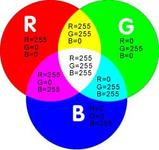
\includegraphics[scale=0.65]{figs/concept_RGB.jpg}
    	\label{ll:ms:rgb}
\end{figure}
\item[CMYK] 油墨对颜色的感知模式。分别对应青色、品红色、黄色和黑色。理想情况下,[100,100,100]代表黑,[0,0,0]代表白。因为无法提取出100\%纯度的CMY三种颜料,所以混合后无法形成纯黑。所以用单独的黑色颜料来代替三者的混合。即现实打印中代表黑的是[0,0,0,100],代表白的是[0,0,0,0]。其他的则是[x,x,x,0]。注意上图\ref{ll:ms:rgb}中,RGB两两混合后即为CMY。
\item[LAB] 大自然对颜色的感知模式。$LAB>CMYK,LAB>RGB$。
\end{description}
\end{enumerate}





\clearpage
%menu
\section{工具[tools]}
\subsection{颜色工具[color tools]}
\subsubsection{色阶[levels]}
\begin{description}
\item[定义]	表示图像亮度强弱的指数标准,也就是我们说的色彩指数,在数字图像处理教程中,指的是灰度分辨率(又称为灰度级分辨率或者幅度分辨率)。图像的色彩丰满度和精细度是由色阶决定的。色阶指亮度和颜色无关,但最亮的只有白色,最不亮的只有黑色。
\item[用途]	表现了一副图的明暗关系.如8位色的RGB空间数字图像,分别用256个阶度表示红绿蓝.
\item[用例]	
\end{description}


\subsubsection{亮度-对比度[brightness-contrast]}
\begin{description}
\item[亮度定义]	指画面的明亮程度
\item[对比度]		是一幅图像中明暗区域最亮的白和最暗的黑之间不同亮度层级的测量,差异范围越大代表对比越大,差异范围越小代表对比越小
\item[用途]	调节图像的明亮程度以及对比度
\item[用例]	
\end{description}


\subsection{其他工具[other tools]}
\subsubsection{路径[paths]}
路径工具可以创建复杂的选区,比如贝兹曲线,它有点像套索,但对所有的矢量曲线都适用。您可以编辑你的曲线,也可以用曲线画画,甚至是保存,导入,导出曲线。您还可以使用路径来创建几何图形。


\clearpage

\section{图像[Image]}
\subsection{复制图像[Duplicate]} 
该命令创建一个新的图像,这是当前图像的一个副本,包含了图像所有图层,通道和路径。 GIMP的剪贴板和历史记录都不会受到影响。

\subsection{平整图像[Flatten Image]}
平整图像命令合并所有图层并将其变成一个没有alpha通道层的单一图像层。图像平整后,它具有和之前相同的外观。所不同的是,所有的图像内容是在一个单一的没有的不透明度的图层。如果透过原始图像的所有图层有任何透明区域,那么那区域的背景颜色是可见的。

此操作使图像的结构发生显着的变化。它通常是当你想要以一种不支持图层和透明(alpha通道)的形式保存时才会用到。

\clearpage


\section{图层[Layer]}
\subsection{透明[Transparency]}
\subsubsection{透明图层到选取[alpha to selection]} 
该命令根据当前图层的alpha通道创建一个选区。不透明区域完全选中,透明区域则不会选中,半透明区域则部分被选中。这种选区将替换现有的选区。 alpha通道本身不会被更改。

在这组操作中其他的命令是相似的,除了完全替换现存的选区,他也可以将两个选取相加,相减或者求两个选区的交集。

\subsection{平整图像[Flatten Image]}
平整图像命令合并所有图层并将其变成一个没有alpha通道层的单一图像层。图像平整后,它具有和之前相同的外观。所不同的是,所有的图像内容是在一个单一的没有的不透明度的图层。如果透过原始图像的所有图层有任何透明区域,那么那区域的背景颜色是可见的。

此操作使图像的结构发生显着的变化。它通常是当你想要以一种不支持图层和透明(alpha通道)的形式保存时才会用到。

\clearpage
%filters
\section{滤镜}
\subsection{模糊滤镜}
简单的模糊滤镜产生一种和相机快门失焦的相似效果,为了产生模糊的特效,该滤镜将该点的像素指和相邻的像素点的值求平均值作为该点的值.
\begin{description}
\item[优点]	计算速度快,适合大图像
\item[缺点]	它的效果在大图像中很难被感知,而在小图像中就很明显
\end{description}
\subsubsection{高斯模糊滤镜}\label{filters:blur:gaussian}
高斯滤镜是应用最广泛的一个模糊滤镜.该滤镜以最基础的方式使得图片更模糊.它能够在相对短的时间里产生一个非常模糊的效果.
高斯滤镜对每个活动图层或者选区都会产生效果,并且会对对话框里定义的范围里所有的像素求平均.\\
对话框参数设置:
\begin{description}
\item[模糊半径]	设置模糊的强烈程度--对于某个像素点,半径越大,求平均的点越多,图片就会越模糊.
\item[模糊方法]	GIMP支持两种高斯滤镜的方式:IIR和RLE.它们都能产生相同的结果,可是在不同情况下,两种方法处理的速度不一样
\begin{description}
\item[IIR]	无限脉冲响应滤波器(Infinite impulse response),该方法适合比较大的模糊半径以及不是电脑生产的图片
\item[RLE]	游程编码(Run-length encoding),该方法适合计算机生成的图片或者[those with large areas of constant intensity.]
\end{description}
\end{description}
高斯滤镜效果比对如下图\ref{filters:blur:gaussian:figure}:
\begin{figure}[!htbp]
	\centering
	\caption{高斯滤镜}
	\subfigure[原图]{
		\label{filters:blur:gaussian:figure:original}
    		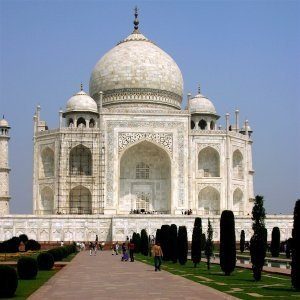
\includegraphics{figs/blur_gaussian_original.jpg}}
    	\subfigure[处理后]{
    		\label{filters:blur:gaussian:figure:dealt}
    		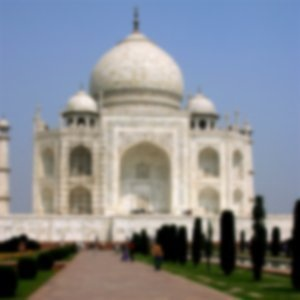
\includegraphics{figs/blur_gaussian_dealt.jpg}}
    	\label{filters:blur:gaussian:figure}
\end{figure}
\clearpage


\subsection{噪声滤镜}
噪声滤镜给可见图层或者选中的选区添加噪音\footnote{图像中各种妨碍人们对其信息接受的因素,详情见http://baike.baidu.com/view/944141.htm}。要是想要除去图片上的小噪点,可以使用降噪\ref{filters:enhance:despeckle}和选择高斯模糊滤镜\ref{filters:blur:selective_gaussian}。

\subsubsection{RGB噪声滤镜}\label{filters:noise:rgb}
RGB噪声滤镜可以给一个图层或一个选区添加符合正态分布的噪声。它利用RGB色彩模式来产生噪音(噪声直接加到每个像素的R,G,B的值上)。正态分布是指只有一小部分像素被很大的值影响,大部分像素只是增加了非常微小的噪声。(如果你对一个填充了灰色的图像进行RGB噪声滤镜后,再看它的直方图,你将看到一个典型的钟形高斯曲线)。而图像中是一个非常自然的噪声。\\
注:\textcolor{red}{该滤镜对索引图像没有效果。}\\
对话框参数设置:
\begin{description}
\item[噪声相关性]	噪声可能是不相关的(additive)或者是相关的(multiplicative - 也被称为斑点噪声)。选中该选项时,每个通道的值乘以一个正态分布值。所以噪声取决于通道值:更大的信道值会导致更多的噪音,而黑色(小值)倾向于保持黑色。
\item[RGB的一致性]	当此按钮被选中时,你可以单独移动每个RGB滑块。否则,三个滑块将一起移动。相关噪声将被添加到每个像素中的所有信道,所以像素的色调不会发生大的变化。
\end{description}
RGB噪声滤镜效果比对如下图\ref{filters:noise:rgb:figure}:
\begin{figure}[!htbp]
	\centering
	\caption{RGB噪声滤镜}
	\subfigure[原图]{
		\label{filters:noise:rgb:figure:original}
    		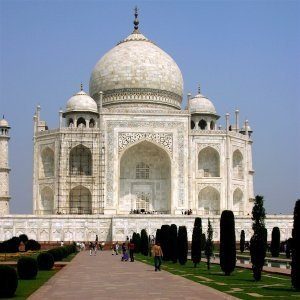
\includegraphics{figs/blur_gaussian_original.jpg}}
    	\subfigure[处理后]{
    		\label{filters:noise:rgb:figure:dealt}
    		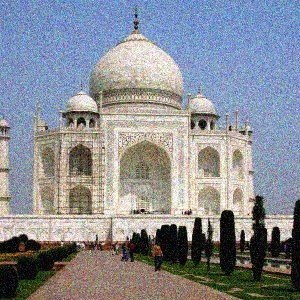
\includegraphics{figs/blur_rgb_dealt.jpg}}
    	\label{filters:noise:rgb:figure}
\end{figure}
\clearpage


\subsection{绘制滤镜}
GIMP的大部分滤镜是通过变换它们的内容作用在一个图层上,但是在绘制这个滤镜中有点不一样。它们从空白开始创建,大部分情况是删除在图层上的任何东西。一些滤镜创建随机或噪图案,其他一些滤镜创建重复的分形图案,还有一个Gfig滤镜是一个专门用来创建矢量图像的工具。

\subsubsection{拼图滤镜}\label{filters:render:pattern:jigsaw}
该滤镜将把你的图片转变成一个拼图。图片边缘有点失真,所以用平滑处理一下会让图片看得更好。\\
\underline{技巧}:如果你想要轻易的选择单个的拼图,你可以在一个填充了白色的单独图层上绘制拼图图案,并且设置图层模式为正片(multiply)。接着你就可以用魔术棒工具在新拼图图层上选择单个拼图。\\
对话框参数设置:
\begin{description}
\item[拼图碎片个数]	设定图片被分为长×宽个拼图碎片。
\item[斜面宽度]	该选项控制拼图碎片边缘的斜率(硬木板拼图需要一个低的斜面宽度值,而软纸板拼图需要更高的值)。
\item[高亮]	该滑块控制高亮的强弱,并且会在每个碎片的边缘体现出来。你可能会将它跟由比较有光泽的材料制成的拼图作比较。高亮宽度值和拼图碎片个数相关。一般,拼图的碎片越多,你应该使用越低的斜率和高亮值,反之亦然。默认值最适合500×500的图片。
\item[拼图风格]	你可以选择两种拼图风格:方块型你将获得由直线构成的碎片;曲线型你将获得由曲线构成的碎片。
\end{description}
jigsaw滤镜效果如下图\ref{filters:render:pattern:jigsaw:figure}
\begin{figure}[!htbp]
	\centering
	\caption{jigsaw滤镜}
	\subfigure[原图]{
		\label{filters:render:pattern:jigsaw:figure:original}
    		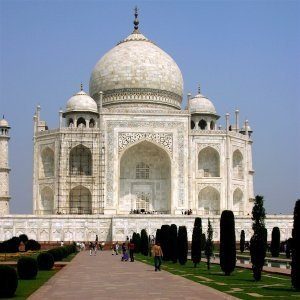
\includegraphics{figs/blur_gaussian_original.jpg}}
    	\subfigure[处理后]{
    		\label{filters:render:pattern:jigsaw:figure:dealt}
    		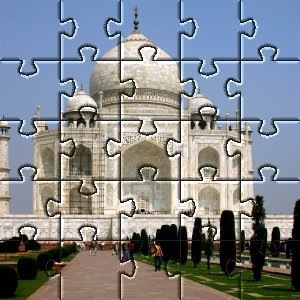
\includegraphics{figs/render_pattern_jigsaw_dealt.jpg}}
    	\label{filters:render:pattern:jigsaw:figure}
\end{figure}
\clearpage


\subsubsection{Gfig滤镜}\label{filters:render:gfig}
Gfig滤镜是一个工具:你可以用它创建几何图形并加入到图片中。当使用这个滤镜的时候,将要被插入到图像中的元素将被放置到一个新的图层。所以原先的图像不会被修改,所有的修改只会作用在新图层。\\
对话框参数设置:
\begin{description}
\item[笔画]	选中该选项时,可以选择颜色以及笔刷。
\item[填充]	选择给对象填充颜色,图案还是渐变。
\end{description}
Gfig滤镜效果如下图\ref{filters:render:gfig:figure}
\begin{figure}[!htbp]
	\centering
	\caption{Gfig滤镜}
	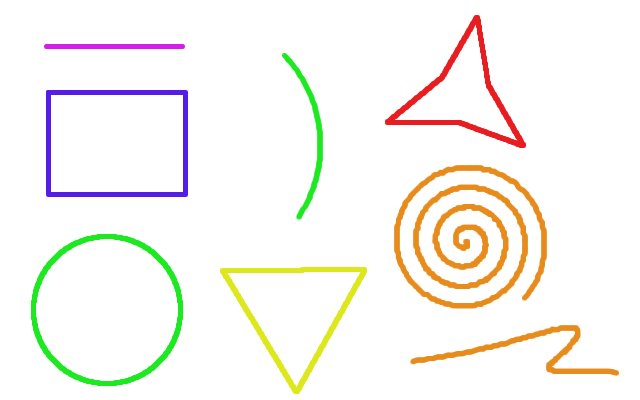
\includegraphics[scale=0.5]{figs/rendering_gfig.jpg} 
    	\label{filters:render:gfig:figure}
\end{figure}






\clearpage
%examples
\section{样例}
\subsection{阴影}\label{yl:yy}
\begin{itemize}
\item 传统操作
\begin{description}
\item[关键点] 三个图层
\begin{description}
\item[背景图层] 一般用白色或透明,用来反衬实景图层
\item[阴影图层] 在实景图层的基础上,用四次高斯模糊滤镜,并往右下方移动4个像素
\item[实景图层] 具体的实景
\end{description}
\item[主要命令] 路径[B],油漆桶填充[shift+B],混合填充[L],移动[M],高斯模糊滤镜
\item[具体操作]
图层结构如下图\ref{yl:yy:layers}:
\begin{figure}[!htbp]
	\centering
	\caption{图层结构}
    	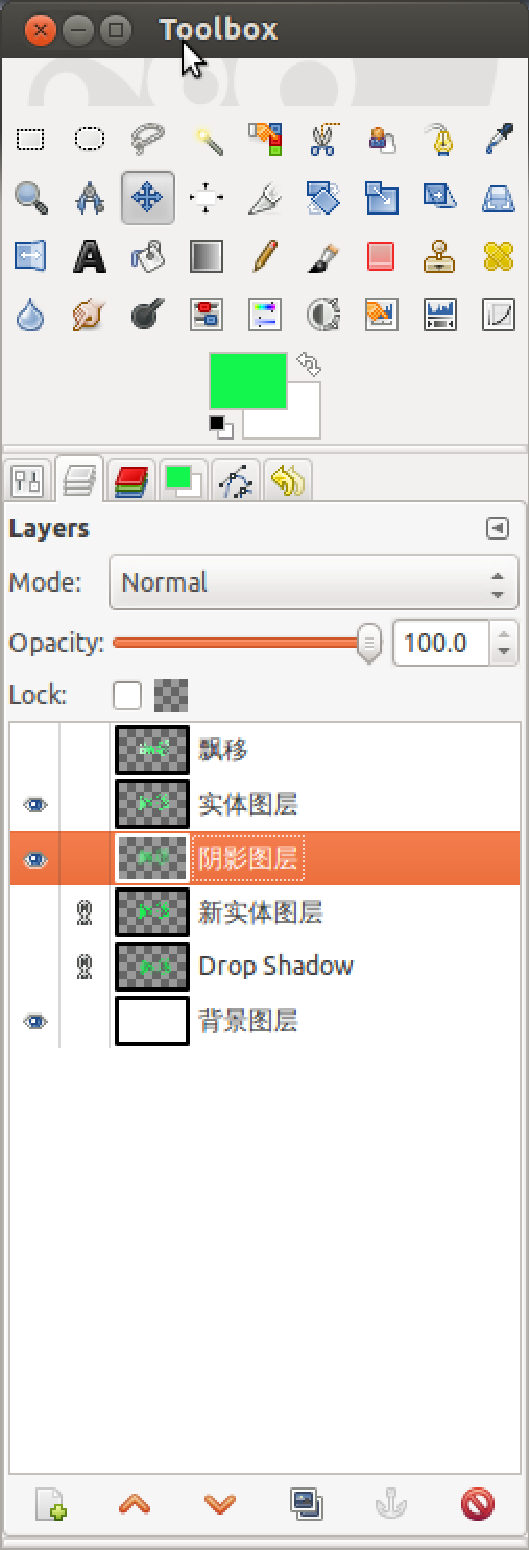
\includegraphics[scale=0.4]{figs/yy-layers.pdf}
    	\label{yl:yy:layers}
\end{figure}
\end{description}
\item 新操作 \\
通过gimp的最新版本中包含的阴影滤镜(drop shadow),可以直接生成阴影.参数设置如下图\ref{yl:yy:set}
\begin{figure}[!htbp]
	\centering
	\caption{阴影滤镜参数设置}
    	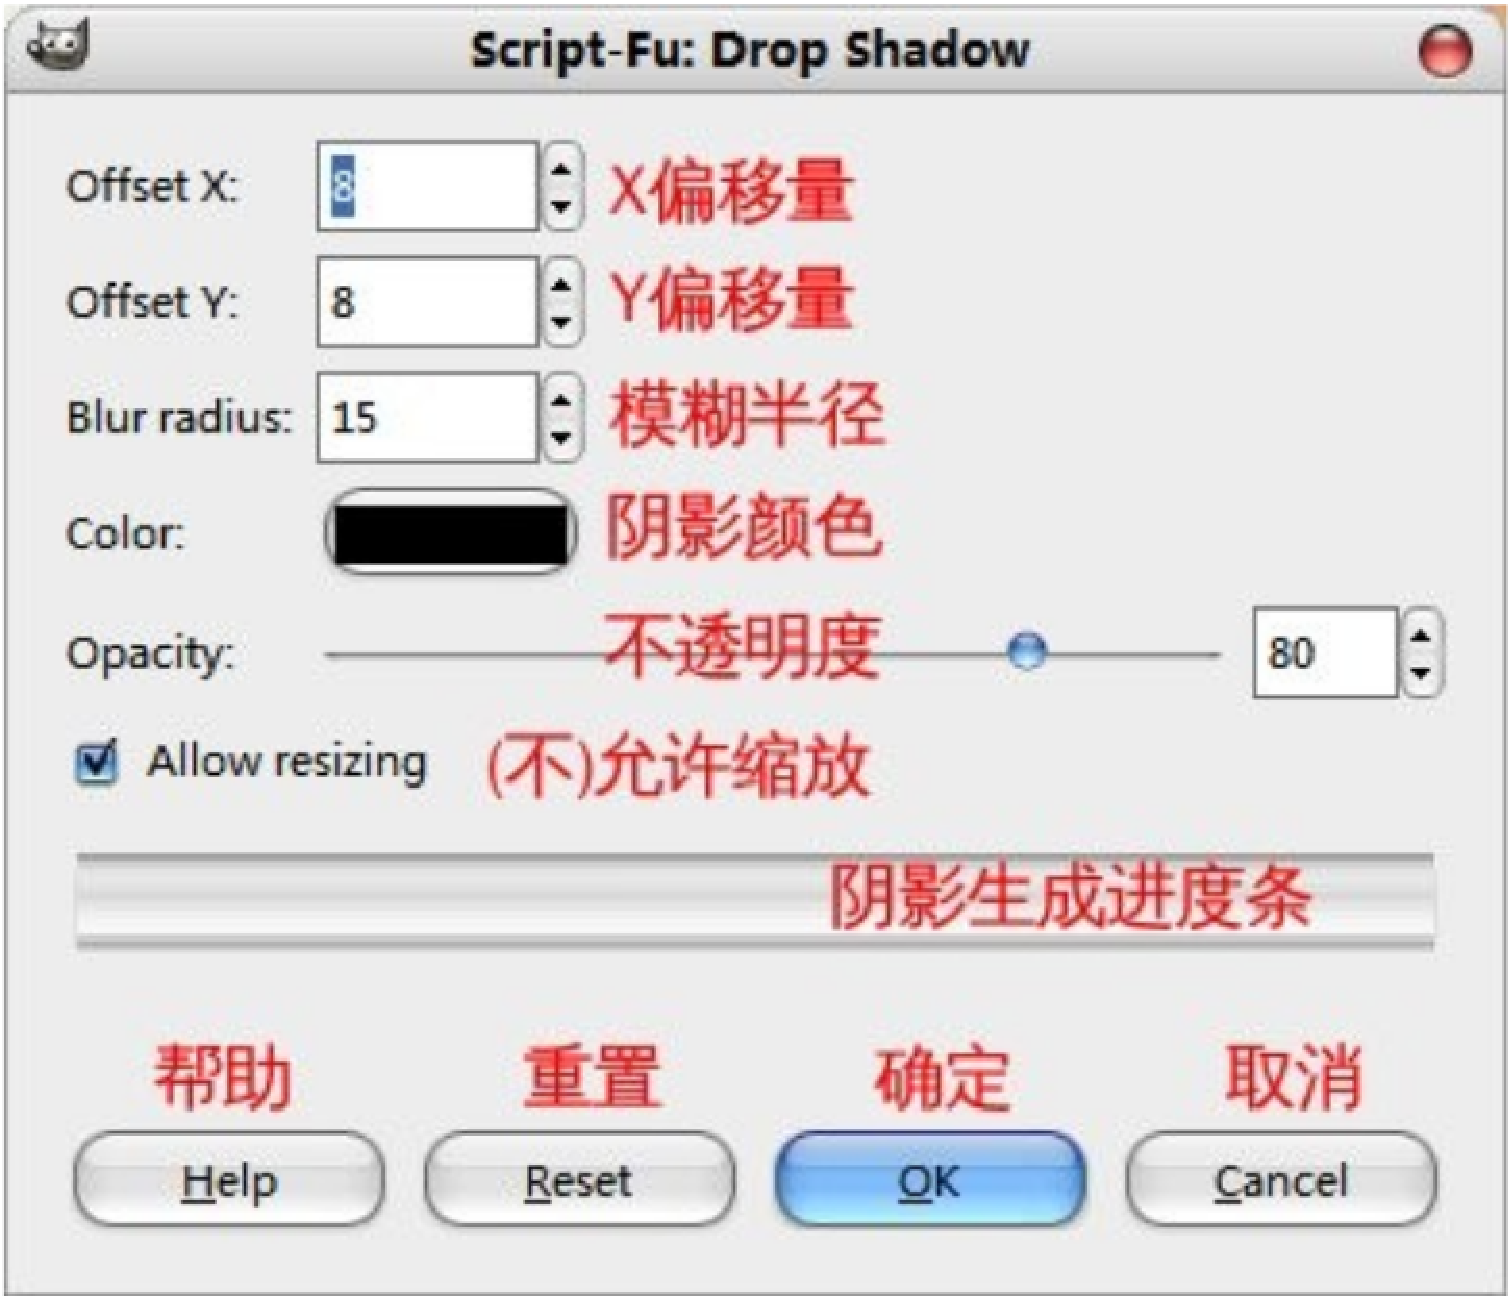
\includegraphics[scale=0.4]{figs/yy-set.pdf}
    	\label{yl:yy:set}
\end{figure}
\end{itemize}

\clearpage

\subsection{金属拉丝}\label{yl:zsls}
\begin{description}
\item[关键点] 
\begin{description}
\item[RGB噪音] 详见RGB噪音\ref{filters:noise:rgb}
\item[高斯模糊] 详见高斯模糊\ref{filters:blur:gaussian}
\end{description}
\item[主要命令] 油漆桶填充[shift+B],高斯模糊,RGB噪音
\item[具体操作]
图层结构如下图\ref{yl:zsls:layers}:
\begin{figure}[!htbp]
	\centering
	\caption{图层结构}
    	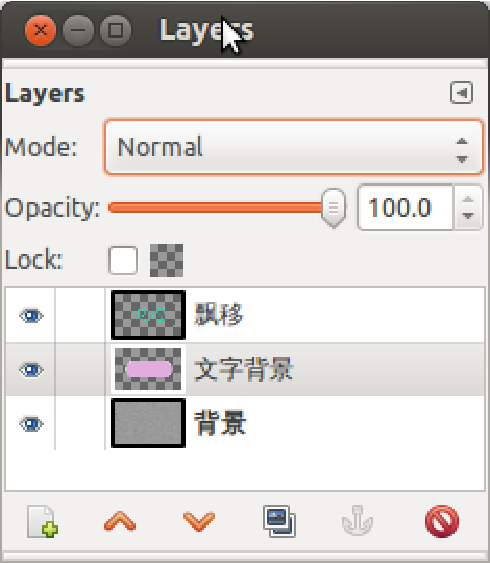
\includegraphics[scale=0.4]{figs/zsls-layers.pdf}
    	\label{yl:zsls:layers}
\end{figure}
效果如下图\ref{yl:zsls:results}:
\begin{figure}[!htbp]
	\centering
	\caption{金属拉丝效果}
    	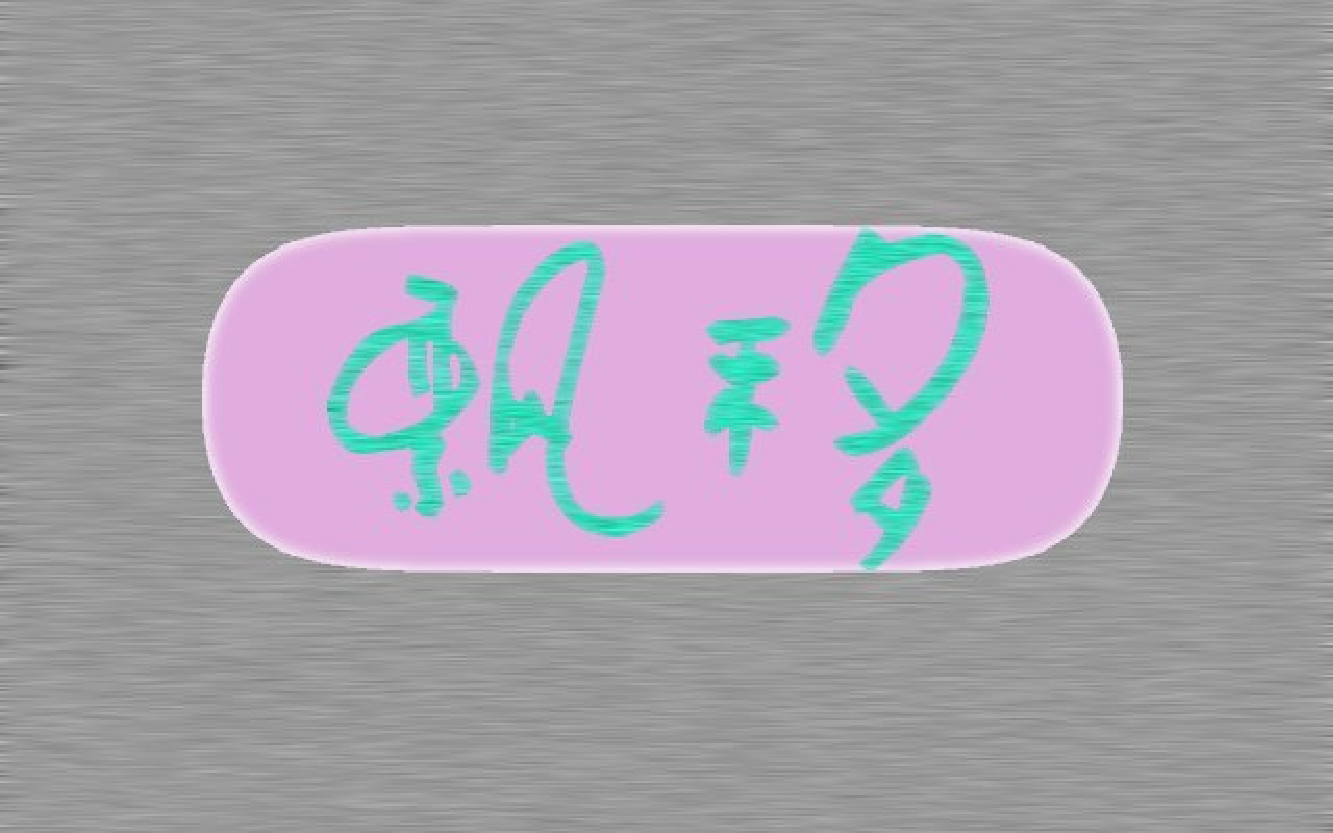
\includegraphics[scale=0.4]{figs/zsls-results.pdf}
    	\label{yl:zsls:results}
\end{figure}
\end{description}





\clearpage


\clearpage     
\end{CJK*}
\end{document}